\documentclass[aspectratio=169]{beamer}
\usepackage[T1]{fontenc}
\usepackage[utf8]{inputenc}
\usepackage{lmodern}
\usepackage{microtype}
\usepackage{xcolor}
\usepackage{tikz}
\usetikzlibrary{positioning, arrows.meta, calc}
\usepackage{fontawesome5}

\definecolor{wurgreen}{HTML}{34B233}
\definecolor{darkgreen}{HTML}{1F6B1E}
\definecolor{darknavy}{HTML}{1A1A2E}
\definecolor{midgray}{HTML}{6B7280}
\definecolor{lightgray}{HTML}{F3F4F6}
\definecolor{lightgreen}{HTML}{E8F7E8}
\definecolor{bodytext}{HTML}{1F2937}
\definecolor{warnred}{HTML}{FEE2E2}
\definecolor{warnborder}{HTML}{EF4444}
\definecolor{codebg}{HTML}{1E1E2E}
\definecolor{codegreen}{HTML}{9ECE6A}
\definecolor{codeblue}{HTML}{7AA2F7}
\definecolor{codegray}{HTML}{C0CAF5}

\usetheme{default}
\usecolortheme{default}
\usefonttheme{professionalfonts}
\setbeamertemplate{navigation symbols}{}
\setbeamertemplate{itemize items}{\textcolor{wurgreen}{\textbullet}}
\setbeamertemplate{itemize subitem}{\textcolor{midgray}{--}}
\setbeamercolor{frametitle}{fg=white, bg=darknavy}
\setbeamerfont{frametitle}{size=\large, series=\bfseries}
\setbeamertemplate{frametitle}{%
  \begin{beamercolorbox}[wd=\paperwidth, ht=1.1cm, dp=0.2cm, leftskip=0.6cm]{frametitle}
    \usebeamerfont{frametitle}\insertframetitle
  \end{beamercolorbox}}
\setbeamercolor{background canvas}{bg=white}
\setbeamercolor{normal text}{fg=bodytext}
\setbeamertemplate{footline}{%
  \begin{beamercolorbox}[wd=\paperwidth, ht=0.4cm, dp=0.15cm]{footline}
    \hspace{0.5cm}\textcolor{midgray}{\tiny Bags, Vectors \& Transformers · Wageningen University \& Research}%
    \hfill\textcolor{midgray}{\tiny \insertframenumber}\hspace{0.4cm}
  \end{beamercolorbox}}

\begin{document}

% ── TITLE ──────────────────────────────────────────────────────────────────
{
\setbeamertemplate{footline}{}
\begin{frame}[plain]
  \begin{tikzpicture}[remember picture, overlay]
    \fill[darknavy] (current page.south west) rectangle (current page.north east);
    \fill[wurgreen] (current page.south west) rectangle
      ([xshift=0.45cm]current page.north west);
    \node[anchor=west, text=white, font=\huge\bfseries, text width=13cm]
      at ([xshift=1.1cm, yshift=1.2cm]current page.west)
      {Bags, Vectors \& Transformers};
    \node[anchor=west, text=wurgreen, font=\large, text width=12cm]
      at ([xshift=1.1cm, yshift=0.05cm]current page.west)
      {Transformers in Practice · Day 3, Part 2};
    \node[anchor=west, text=midgray, font=\small, text width=12cm]
      at ([xshift=1.1cm, yshift=-1.5cm]current page.west)
      {Denise J. Roth, PhD Candidate\\
       Strategic Communication Group · Wageningen University \& Research};
  \end{tikzpicture}
\end{frame}
}

% ── SLIDE 1: roadmap ──────────────────────────────────────────────────────
\begin{frame}{From Theory to Practice}
\vspace{0.2cm}
{\small We know \emph{what} transformers are and \emph{how} attention works. Now the questions
that matter for actually \textbf{doing research} with them:}

\medskip
\begin{itemize}\setlength\itemsep{7pt}
  \item[\textcolor{wurgreen}{\faLayerGroup}]
    The \textbf{pre-train then fine-tune} paradigm --- why it changes everything
  \item[\textcolor{wurgreen}{\faWrench}]
    Three ways to \textbf{use} a pre-trained model
  \item[\textcolor{wurgreen}{\faSlidersH}]
    Practical \textbf{parameters}: model size, sequence length, variants
  \item[\textcolor{wurgreen}{\faGlobeEurope}]
    Models for \textbf{other languages} (including Dutch)
  \item[\textcolor{wurgreen}{\faRocket}]
    \textbf{Hugging Face}: how you actually load one in a few lines
\end{itemize}

\medskip
{\small\textcolor{midgray}{\textit{Then straight into the notebook.}}}
\end{frame}

% ── SLIDE 2: pretrain/finetune paradigm ───────────────────────────────────
\begin{frame}{The Big Idea: Pre-train Once, Fine-tune Often}
\vspace{0.2cm}
{\small The reason transformers are usable by \emph{everyone}, not just big labs, is a
two-stage split:}

\medskip
\begin{center}
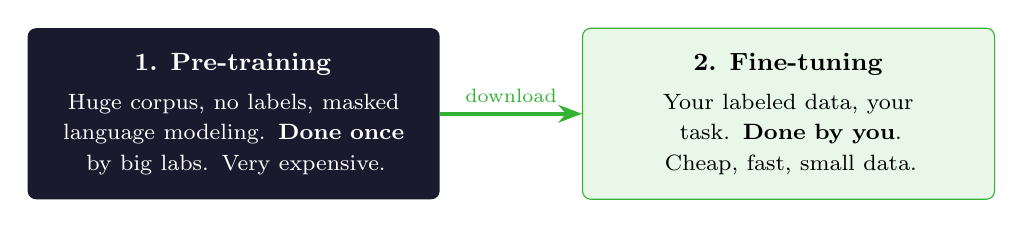
\begin{tikzpicture}[font=\small, node distance=1.2cm]
  \node[fill=darknavy, rounded corners=3pt, inner sep=9pt, text width=4.6cm, align=center] (pre)
    {\textcolor{white}{\textbf{1. Pre-training}}\\[3pt]
     {\footnotesize\color{white} Huge corpus, no labels, masked language modeling.
     \textbf{Done once} by big labs. Very expensive.}};
  \node[fill=lightgreen, draw=wurgreen, rounded corners=3pt, inner sep=9pt,
        text width=4.6cm, align=center, right=1.8cm of pre] (fine)
    {\textbf{2. Fine-tuning}\\[3pt]
     {\footnotesize Your labeled data, your task. \textbf{Done by you}.
     Cheap, fast, small data.}};
  \draw[-{Stealth[length=3mm]}, wurgreen, line width=1.3pt] (pre) -- (fine)
    node[midway, above, font=\scriptsize] {download};
\end{tikzpicture}
\end{center}

\medskip
{\small The model arrives already knowing \textbf{how language works} (grammar, meaning, world
knowledge). You just \textbf{nudge} it toward your specific task with a modest amount of
labeled examples. This is called \textbf{transfer learning}.}
\end{frame}

% ── SLIDE 3: why fine-tuning is powerful ──────────────────────────────────
\begin{frame}{Why Fine-tuning Is a Big Deal for Social Science}
\vspace{0.3cm}
\begin{columns}[T]
  \column{0.48\textwidth}
  \vspace{0pt}
  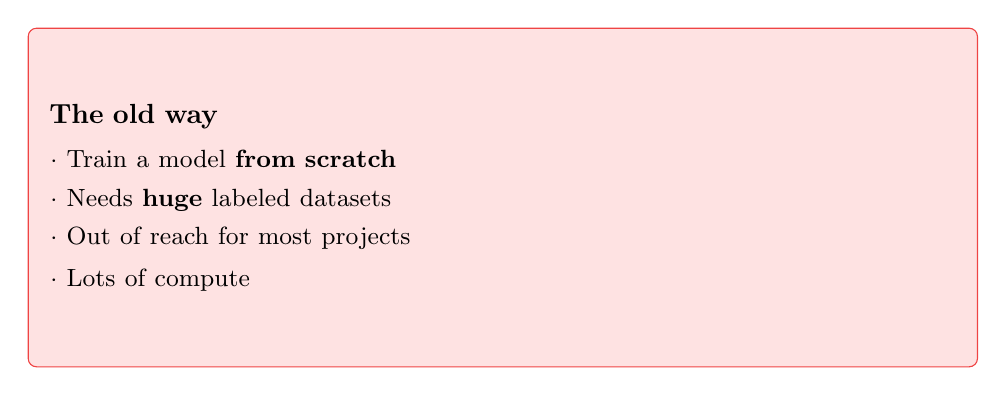
\begin{tikzpicture}
    \node[fill=warnred, draw=warnborder, rounded corners=3pt,
          inner xsep=8pt, inner ysep=8pt, text width=\columnwidth-18pt, minimum height=4.3cm]{%
      \textbf{The old way}\\[5pt]
      {\small
      $\cdot$ Train a model \textbf{from scratch}\\[3pt]
      $\cdot$ Needs \textbf{huge} labeled datasets\\[3pt]
      $\cdot$ Out of reach for most projects\\[3pt]
      $\cdot$ Lots of compute}};
  \end{tikzpicture}

  \column{0.48\textwidth}
  \vspace{0pt}
  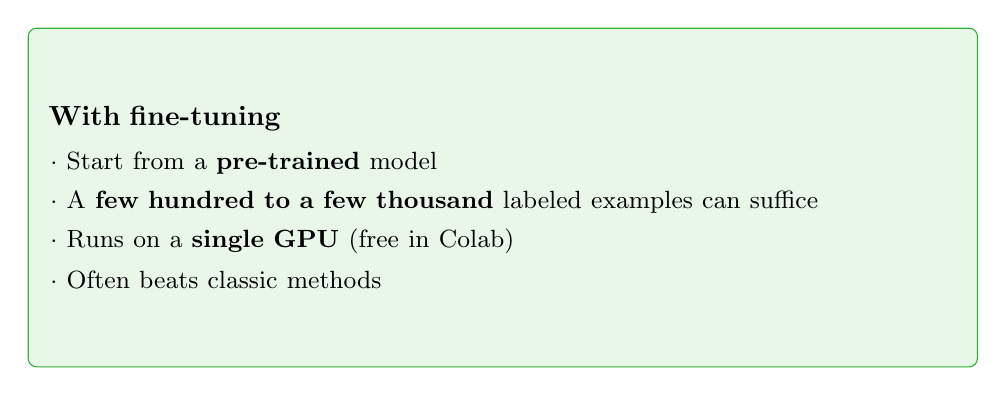
\begin{tikzpicture}
    \node[fill=lightgreen, draw=wurgreen, rounded corners=3pt,
          inner xsep=8pt, inner ysep=8pt, text width=\columnwidth-18pt, minimum height=4.3cm]{%
      \textbf{With fine-tuning}\\[5pt]
      {\small
      $\cdot$ Start from a \textbf{pre-trained} model\\[3pt]
      $\cdot$ A \textbf{few hundred to a few thousand} labeled examples can suffice\\[3pt]
      $\cdot$ Runs on a \textbf{single GPU} (free in Colab)\\[3pt]
      $\cdot$ Often beats classic methods}};
  \end{tikzpicture}
\end{columns}

\medskip
{\small\textcolor{midgray}{\textit{Hand-labeling 500 documents is a realistic afternoon.
Hand-labeling a million is not. Fine-tuning meets you where your data is.}}}
\end{frame}

% ── SLIDE 4: three ways to use ────────────────────────────────────────────
\begin{frame}{Three Ways to Use a Pre-trained Model}
\vspace{0.2cm}
\begin{columns}[T]
  \column{0.32\textwidth}
  \vspace{0pt}
  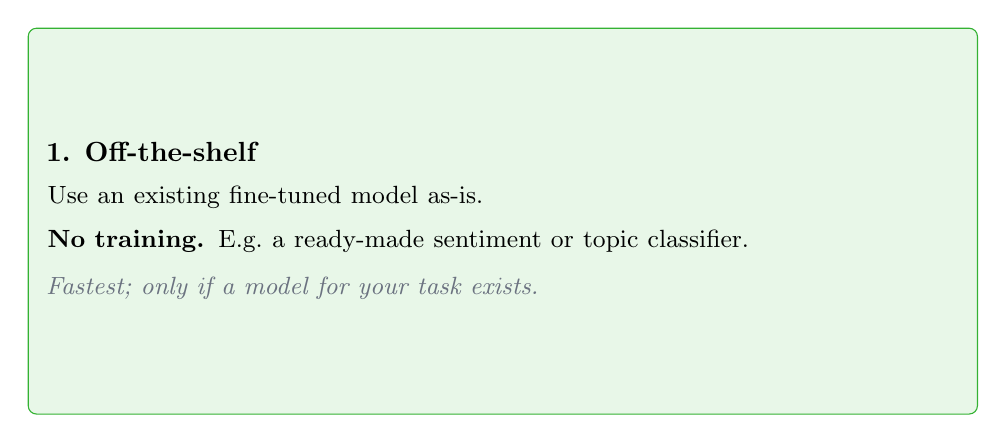
\begin{tikzpicture}
    \node[fill=lightgreen, draw=wurgreen, rounded corners=3pt,
          inner xsep=7pt, inner ysep=8pt, text width=\columnwidth-16pt, minimum height=4.9cm]{%
      \textbf{1. Off-the-shelf}\\[4pt]
      {\small Use an existing fine-tuned model as-is.\\[5pt]
      \textbf{No training.} E.g.\ a ready-made sentiment or topic classifier.\\[5pt]
      \textcolor{midgray}{\textit{Fastest; only if a model for your task exists.}}}};
  \end{tikzpicture}

  \column{0.32\textwidth}
  \vspace{0pt}
  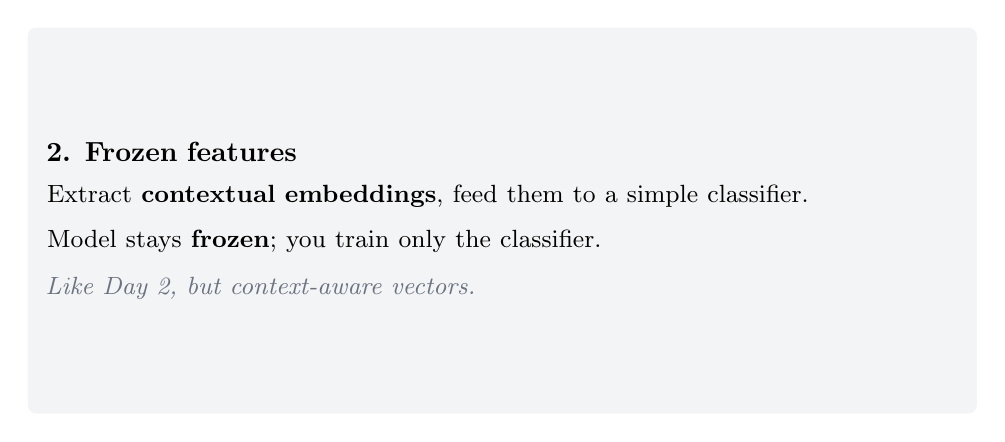
\begin{tikzpicture}
    \node[fill=lightgray, rounded corners=3pt,
          inner xsep=7pt, inner ysep=8pt, text width=\columnwidth-16pt, minimum height=4.9cm]{%
      \textbf{2. Frozen features}\\[4pt]
      {\small Extract \textbf{contextual embeddings}, feed them to a simple classifier.\\[5pt]
      Model stays \textbf{frozen}; you train only the classifier.\\[5pt]
      \textcolor{midgray}{\textit{Like Day 2, but context-aware vectors.}}}};
  \end{tikzpicture}

  \column{0.32\textwidth}
  \vspace{0pt}
  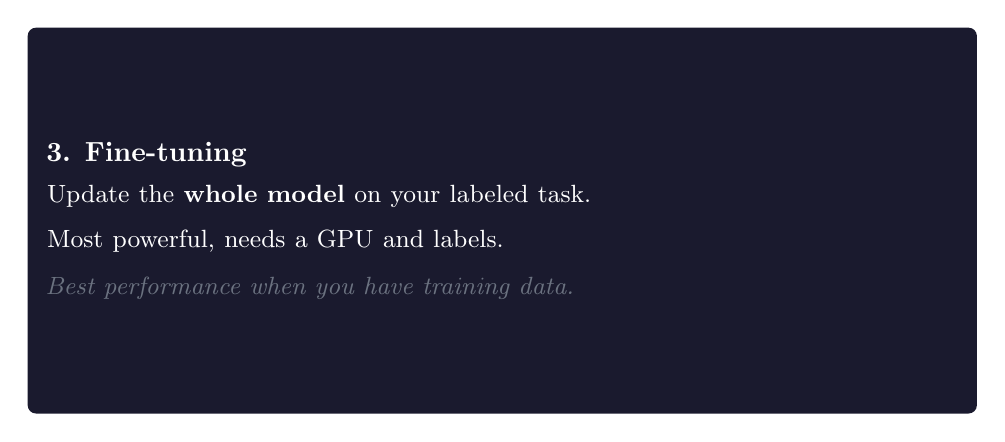
\begin{tikzpicture}
    \node[fill=darknavy, rounded corners=3pt,
          inner xsep=7pt, inner ysep=8pt, text width=\columnwidth-16pt, minimum height=4.9cm]{%
      \textcolor{white}{\textbf{3. Fine-tuning}}\\[4pt]
      {\small\color{white} Update the \textbf{whole model} on your labeled task.\\[5pt]
      Most powerful, needs a GPU and labels.\\[5pt]
      \color{midgray}\textit{Best performance when you have training data.}}};
  \end{tikzpicture}
\end{columns}

\medskip
{\small\textcolor{midgray}{\textit{Increasing effort, increasing power --- left to right. Pick
the lightest one that solves your problem.}}}
\end{frame}

% ── SLIDE 5: what to use them for ─────────────────────────────────────────
\begin{frame}{What Can You Use Them For?}
\vspace{0.3cm}
\begin{columns}[T]
  \column{0.48\textwidth}
  \vspace{0pt}
  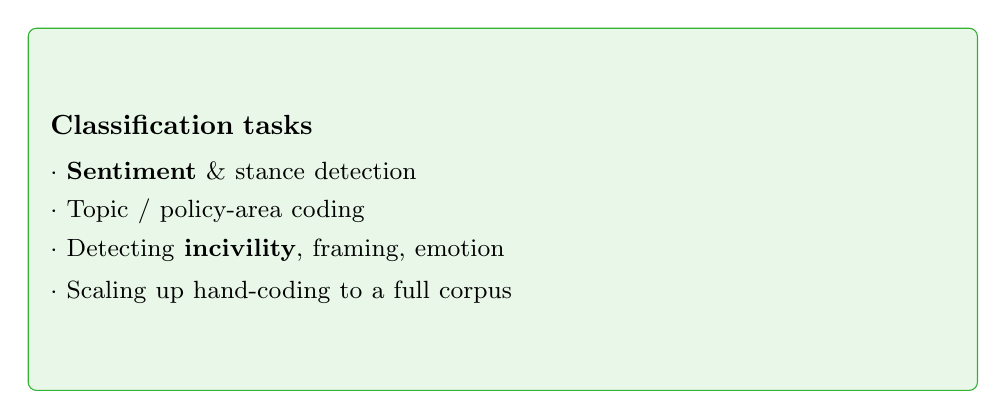
\begin{tikzpicture}
    \node[fill=lightgreen, draw=wurgreen, rounded corners=3pt,
          inner xsep=8pt, inner ysep=8pt, text width=\columnwidth-18pt, minimum height=4.6cm]{%
      \textbf{Classification tasks}\\[5pt]
      {\small
      $\cdot$ \textbf{Sentiment} \& stance detection\\[3pt]
      $\cdot$ Topic / policy-area coding\\[3pt]
      $\cdot$ Detecting \textbf{incivility}, framing, emotion\\[3pt]
      $\cdot$ Scaling up hand-coding to a full corpus}};
  \end{tikzpicture}

  \column{0.48\textwidth}
  \vspace{0pt}
  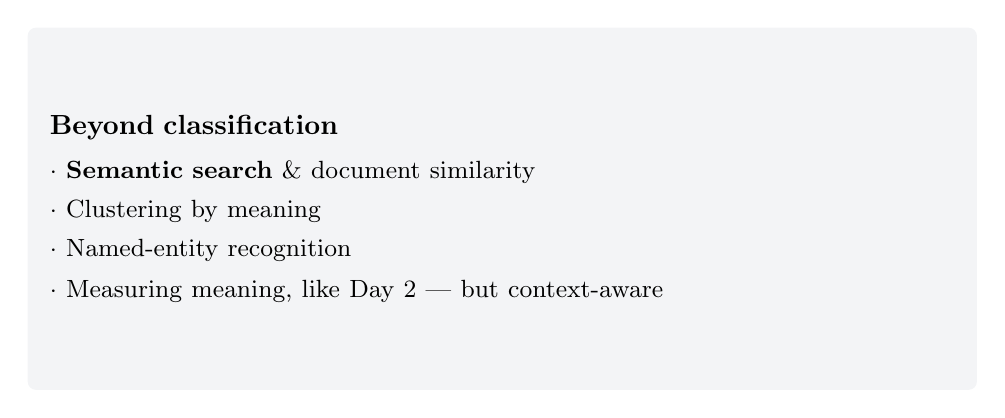
\begin{tikzpicture}
    \node[fill=lightgray, rounded corners=3pt,
          inner xsep=8pt, inner ysep=8pt, text width=\columnwidth-18pt, minimum height=4.6cm]{%
      \textbf{Beyond classification}\\[5pt]
      {\small
      $\cdot$ \textbf{Semantic search} \& document similarity\\[3pt]
      $\cdot$ Clustering by meaning\\[3pt]
      $\cdot$ Named-entity recognition\\[3pt]
      $\cdot$ Measuring meaning, like Day 2 --- but context-aware}};
  \end{tikzpicture}
\end{columns}

\medskip
{\small\textcolor{midgray}{\textit{The common thread: any task where you would otherwise
hand-read thousands of documents.}}}
\end{frame}

% ── SLIDE 6: practical parameters ─────────────────────────────────────────
\begin{frame}{Practical Parameters to Know}
\vspace{0.2cm}
\begin{columns}[T]
  \column{0.48\textwidth}
  \vspace{0pt}
  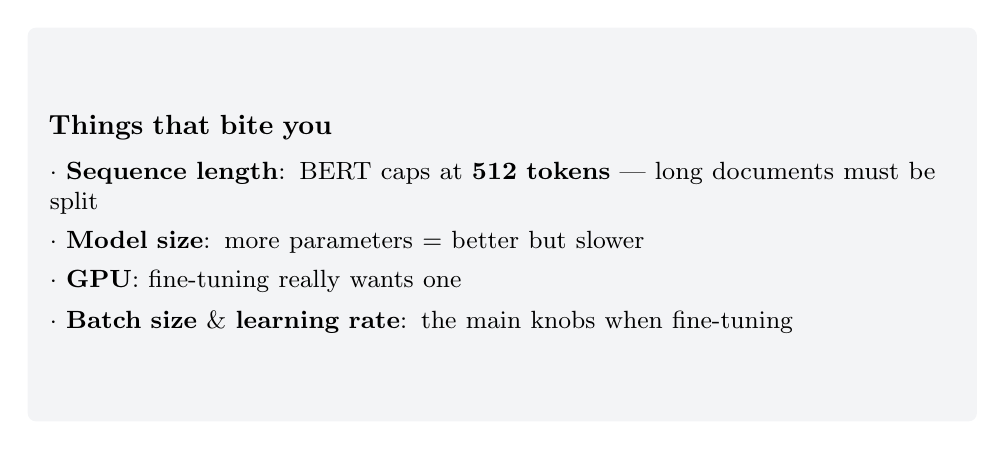
\begin{tikzpicture}
    \node[fill=lightgray, rounded corners=3pt,
          inner xsep=8pt, inner ysep=8pt, text width=\columnwidth-18pt, minimum height=5cm]{%
      \textbf{Things that bite you}\\[5pt]
      {\small
      $\cdot$ \textbf{Sequence length}: BERT caps at \textbf{512 tokens} --- long documents must be split\\[3pt]
      $\cdot$ \textbf{Model size}: more parameters = better but slower\\[3pt]
      $\cdot$ \textbf{GPU}: fine-tuning really wants one\\[3pt]
      $\cdot$ \textbf{Batch size} \& \textbf{learning rate}: the main knobs when fine-tuning}};
  \end{tikzpicture}

  \column{0.48\textwidth}
  \vspace{0pt}
  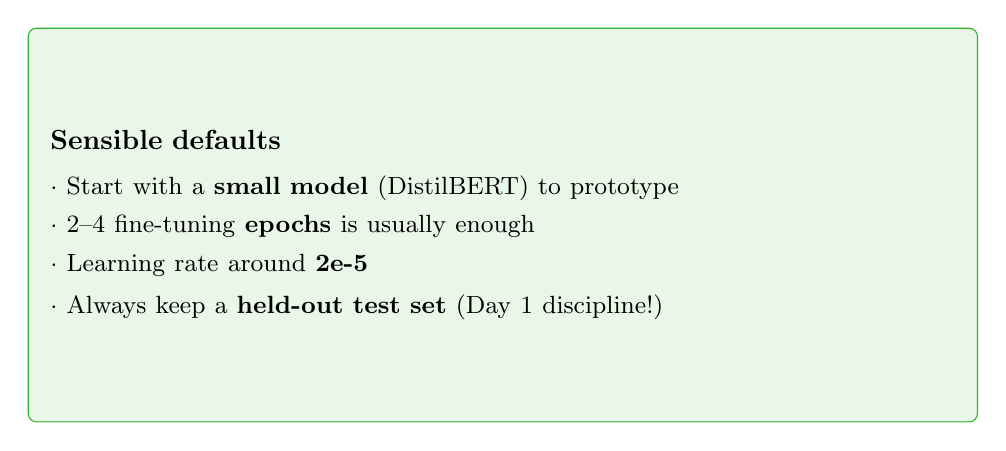
\begin{tikzpicture}
    \node[fill=lightgreen, draw=wurgreen, rounded corners=3pt,
          inner xsep=8pt, inner ysep=8pt, text width=\columnwidth-18pt, minimum height=5cm]{%
      \textbf{Sensible defaults}\\[5pt]
      {\small
      $\cdot$ Start with a \textbf{small model} (DistilBERT) to prototype\\[3pt]
      $\cdot$ 2--4 fine-tuning \textbf{epochs} is usually enough\\[3pt]
      $\cdot$ Learning rate around \textbf{2e-5}\\[3pt]
      $\cdot$ Always keep a \textbf{held-out test set} (Day 1 discipline!)}};
  \end{tikzpicture}
\end{columns}
\end{frame}

% ── SLIDE 7: model variants ───────────────────────────────────────────────
\begin{frame}{A Family of Models}
\vspace{0.2cm}
{\small ``BERT'' is really a whole family. You rarely need the original --- pick the variant
that fits your constraints.}

\medskip
\begin{center}
\renewcommand{\arraystretch}{1.35}
{\small
\begin{tabular}{p{2.6cm}|p{9.5cm}}
\textbf{BERT} & the original; solid general-purpose baseline \\
\textbf{RoBERTa} & better-trained BERT; often higher accuracy \\
\textbf{DistilBERT} & smaller \& faster ($\sim$40\% lighter), minimal accuracy loss --- great for prototyping \\
\textbf{mBERT / XLM-R} & \textbf{multilingual}; one model, 100+ languages \\
\textbf{BERTje / RobBERT} & \textbf{Dutch} models, trained on Dutch text \\
\end{tabular}
}
\end{center}

\medskip
{\small\textcolor{midgray}{\textit{For Dutch social-science data, \textbf{BERTje} or
\textbf{RobBERT} will usually beat a multilingual model --- and both are a click away.}}}
\end{frame}

% ── SLIDE 8: hugging face ─────────────────────────────────────────────────
\begin{frame}{Hugging Face: The Practical Gateway}
\vspace{0.2cm}
{\small You do not train these from scratch or hunt down files. \textbf{Hugging Face} is a hub
of \textbf{thousands of pre-trained models}, plus the \texttt{transformers} library to use
them.}

\medskip
\begin{columns}[T]
  \column{0.46\textwidth}
  \vspace{0pt}
  \begin{tikzpicture}
    \node[fill=lightgreen, draw=wurgreen, rounded corners=3pt,
          inner xsep=8pt, inner ysep=8pt, text width=\columnwidth-18pt, minimum height=3.8cm]{%
      \textbf{The Model Hub \faExternalLinkAlt}\\[5pt]
      {\small
      $\cdot$ Search by \textbf{task} or \textbf{language}\\[3pt]
      $\cdot$ Ready-made \& fine-tuned models\\[3pt]
      $\cdot$ Model cards document training \& limits\\[3pt]
      $\cdot$ Mostly free to download}};
  \end{tikzpicture}

  \column{0.5\textwidth}
  \vspace{0pt}
  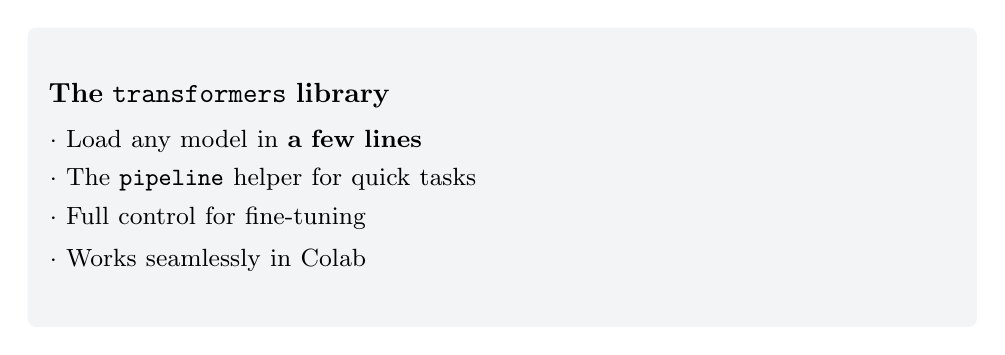
\begin{tikzpicture}
    \node[fill=lightgray, rounded corners=3pt,
          inner xsep=8pt, inner ysep=8pt, text width=\columnwidth-18pt, minimum height=3.8cm]{%
      \textbf{The \texttt{transformers} library}\\[5pt]
      {\small
      $\cdot$ Load any model in \textbf{a few lines}\\[3pt]
      $\cdot$ The \texttt{pipeline} helper for quick tasks\\[3pt]
      $\cdot$ Full control for fine-tuning\\[3pt]
      $\cdot$ Works seamlessly in Colab}};
  \end{tikzpicture}
\end{columns}
\end{frame}

% ── SLIDE 9: code teaser ──────────────────────────────────────────────────
\begin{frame}{Sentiment in Three Lines}
\vspace{0.3cm}
{\small The \texttt{pipeline} helper hides all the complexity. Here is a working
off-the-shelf sentiment classifier:}

\medskip
\begin{center}
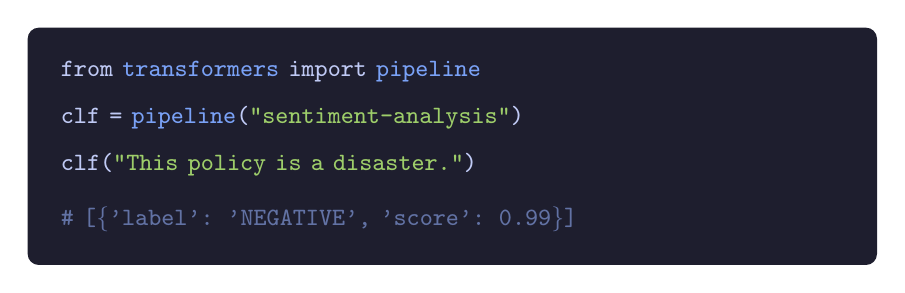
\begin{tikzpicture}
  \node[fill=codebg, rounded corners=4pt, inner sep=12pt, text width=0.82\textwidth,
        text=codegray]{%
    \ttfamily\small
    \textcolor{codegray}{from} \textcolor{codeblue}{transformers} \textcolor{codegray}{import} \textcolor{codeblue}{pipeline}\\[6pt]
    clf \textcolor{codegray}{=} \textcolor{codeblue}{pipeline}(\textcolor{codegreen}{"sentiment-analysis"})\\[6pt]
    clf(\textcolor{codegreen}{"This policy is a disaster."})\\[8pt]
    \textcolor[HTML]{6272A4}{\# [\{'label': 'NEGATIVE', 'score': 0.99\}]}%
  };
\end{tikzpicture}
\end{center}

\medskip
{\small That is a real, state-of-the-art model running on your text. Swapping
\texttt{"sentiment-analysis"} for another task, or naming a specific model (say a Dutch one),
is all it takes to change what it does.}
\end{frame}

% ── SLIDE 10: recap + to notebook ─────────────────────────────────────────
\begin{frame}{Practice: The Takeaways}
\vspace{0.25cm}
\begin{itemize}\setlength\itemsep{7pt}
  \item[\textcolor{wurgreen}{\faCheck}]
    \textbf{Pre-train once, fine-tune often}: the model already knows language; you adapt it cheaply
  \item[\textcolor{wurgreen}{\faCheck}]
    Three usage modes: \textbf{off-the-shelf}, \textbf{frozen features}, \textbf{fine-tuning} ---
    lightest that works
  \item[\textcolor{wurgreen}{\faCheck}]
    Mind the \textbf{512-token limit}, model size, and the need for a GPU when fine-tuning
  \item[\textcolor{wurgreen}{\faCheck}]
    Pick the right \textbf{variant} --- DistilBERT to prototype, \textbf{BERTje/RobBERT} for Dutch
  \item[\textcolor{wurgreen}{\faCheck}]
    \textbf{Hugging Face} makes all of this a few lines of code
\end{itemize}

\medskip
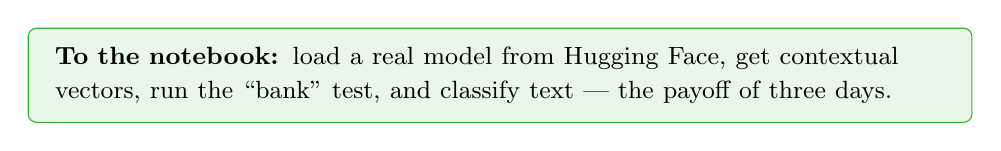
\begin{tikzpicture}
  \node[fill=lightgreen, draw=wurgreen, rounded corners=3pt,
        inner xsep=10pt, inner ysep=7pt, text width=\textwidth-24pt]{%
    {\small \textbf{To the notebook:} load a real model from Hugging Face, get contextual
    vectors, run the ``bank'' test, and classify text --- the payoff of three days.}};
\end{tikzpicture}
\end{frame}

\end{document}
